%!TEX root = ../../../super_main.tex

\section{Missing Apps in Application Grid}
\label{sec:missing_apps_racecondition}

We revealed an issue in the application grid, specifically with the background tasks that loads the applications and their icons. The application grid in the \launcher's Homeactivity would sometimes not show the applications. This issue occurs when the \launcher is to load its applications upon startup. The \launcher starts a background task in its onResume method which loads and prepares the applications to be shown.\\

This bug happens when the onResume method of the Homeactivity checks a boolean variable called \androidinline{mIsAppsContainerInitialized}, which was used in the previous solution to populating the application grid (see \secref{sec:reengineering_of_application_grid}). The previous solution included rebuilding a complicated layout called \androidinline{AppsContainer}, based on \androidinline{LinearLayout} objects, every time the grid had to change. This layout was built on a background thread in a \androidinline{LoadHomeActivityApplicationTask}. Once the layout was completed on the background thread, the variable mIsAppsContainerInitialized was set to true. A check on the variable was then performed to verify whether or not the application screen should be reloaded.

\begin{figure}[!htbp]
    \centering
    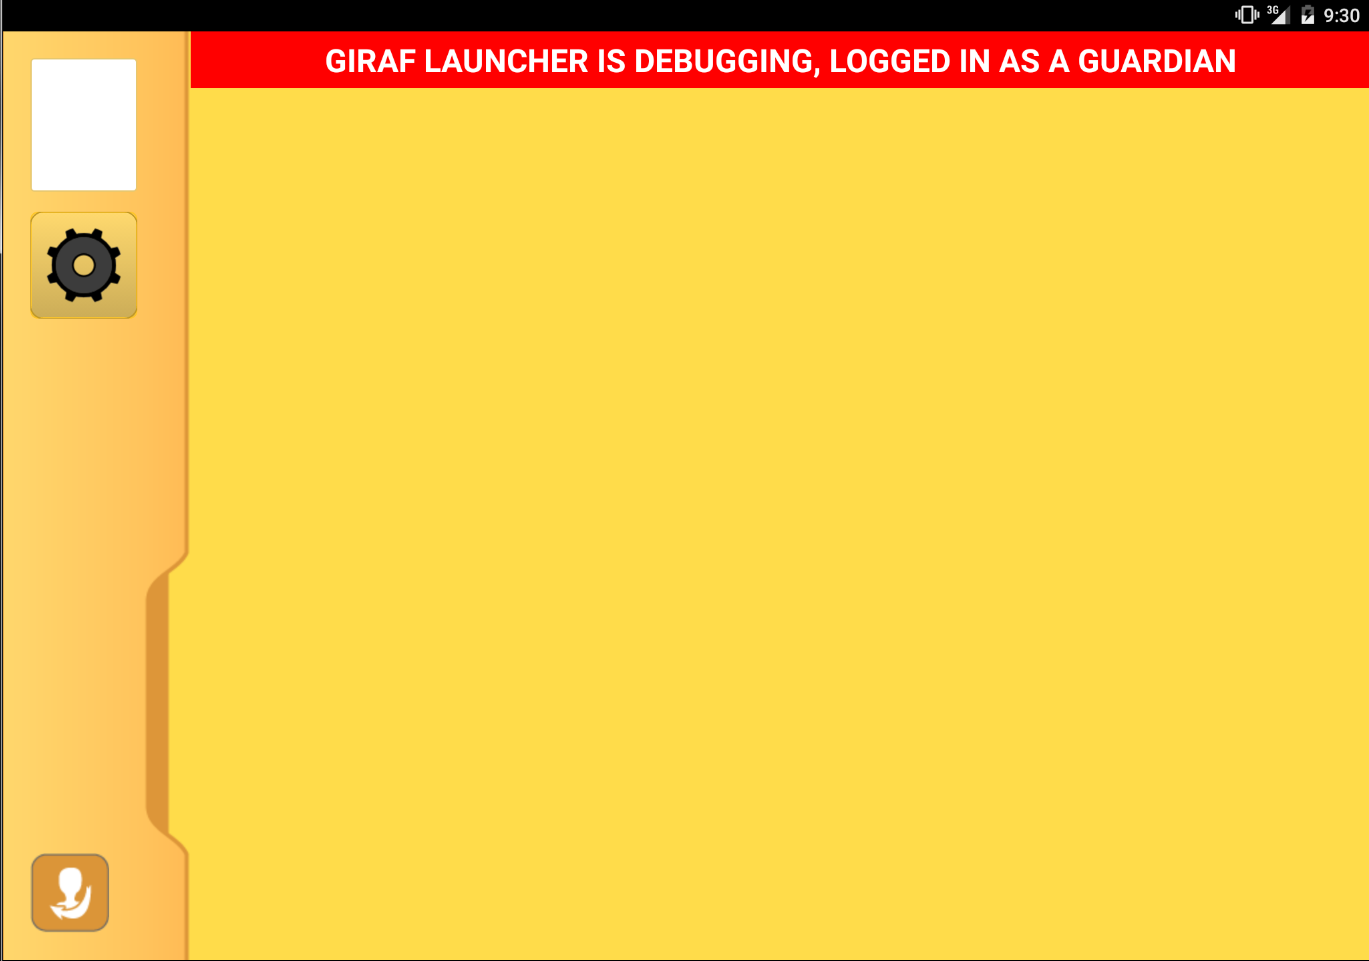
\includegraphics[width=\textwidth]{sprint_one/missing_app_icons/empty_app_icon_screen}
    \caption{Missing Apps}
    \label{fig:missing_apps}
\end{figure}

\subsection{Solution}
\label{sub:missing_apps_racecondition_solution}

The check on \androidinline{mIsAppsContainerInitialized} still happened after we implemented the changes described in \secref{sec:reengineering_of_application_grid}, as it did not seem to have any effect in most cases. Since it has been discovered that errors sometimes happen because of this check, and we no longer have any need to verify that we are done building any layouts, the piece of code has been removed. 